\documentclass{beamer}
 
\usepackage[utf8]{inputenc}
\usepackage{siunitx}
\usetheme{CambridgeUS}
\useinnertheme{circles}

\usefonttheme[onlymath]{serif} 
 
%Information to be included in the title page:

\title{Seminar 5}
\subtitle{General relativity}

\author{Will Barker\inst{1}\inst{2}}
\institute{
  \inst{1}%
    Cavendish Laboratory\\
    University of Cambridge\\
  \inst{2}%
    Kavli Institute for Cosmology\\
    University of Cambridge\\
}
\date{}
\logo{%
  \makebox[0.95\paperwidth]{%
    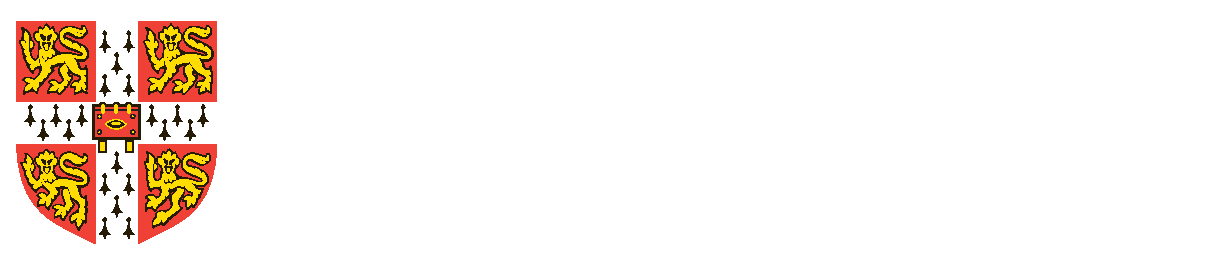
\includegraphics[height=0.7cm,keepaspectratio]{CU.eps}%
    \hfill%
    \includegraphics[height=0.7cm,keepaspectratio]{logo.png}%
  }%
}
 
 
 
\begin{document}
 
\frame{\titlepage}
 
\begin{frame}
  \frametitle{What is general relativity?}
  \begin{itemize}
    \item<1-> Which was invented first, \textbf{special relativity} or \textbf{general relativity}? 
    \item<2-> \textbf{Special relativity} tells us about the \textbf{fundamental structure} of spacetime (\textbf{Minkowskian signature}, \textbf{four dimensions} etc)
    \item<3-> \textbf{General relativity} tells us how the \textbf{geometry} of the spacetime is affected by \textbf{matter}
  \end{itemize}
\end{frame}

\begin{frame}
  \frametitle{High-speed tour of general relativity}
  \begin{itemize}
    \item<1-> Yesterday you studied how spacetime is deformed depending on your velocity
    \item<2-> \textbf{In fact, the principles you derived are about as hard as special relativity gets!}
    \item<3-> Unfortunately, general relativity is \textbf{unbelievably more complicated}\ldots
    \item<4-> In the second part of the seminar, you will derive some interesting properties of \textbf{black holes} and \textbf{gravitational waves}
    \item<5-> To start off, I'll try to give an overview of the physics
    \item<6-> \textbf{FEEL FREE TO HAVE A NAP IF YOU AREN'T INTERESTED: IT IS FRIDAY\ldots}
  \end{itemize}
\end{frame}

\begin{frame}
  \frametitle{High-speed tour of general relativity}
  \begin{itemize}
    \item<1-> The first thing is to understand what we mean by \textbf{curved spacetime}
    \item<2-> Let's say a photon moves through $\Delta t$ in time and $\Delta x$, $\Delta y$ and $\Delta z$ in space\ldots
    \item<3-> What was the formula with squares and a square-root that the photon obeyed in \textbf{special relativity}, which didn't change with $v$?
    \item<4-> We had:
      \begin{equation*}
	\sqrt{c^2\Delta t^2-\Delta x^2-\Delta y^2-\Delta z^2}=0
      \end{equation*}
    \item<5-> \textbf{Square it}!
  \end{itemize}
\end{frame}

\begin{frame}
  \frametitle{High-speed tour of general relativity}
  \begin{itemize}
    \item<1-> Ok, so a \textbf{photon} does this in \textbf{flat} spacetime:
      \begin{equation*}
	c^2\Delta t^2-\Delta x^2-\Delta y^2-\Delta z^2=0
      \end{equation*}
    \item<2-> We also learned that the LHS means \textbf{distance} in special relativity, right?
    \item<3-> What do they tell you about how \textbf{light} travels in school?
    \item<4-> And what is the \textbf{shortest distance} between two points in geometry? 
    \item<5-> OK, so the equation we have is just a mathematical statement of the \textbf{shortest distance}!
  \end{itemize}
\end{frame}

\begin{frame}
  \frametitle{High-speed tour of general relativity}
  \begin{itemize}
    \item<1-> If spacetime is \textbf{curved}, the \textbf{shortest distance} isn't a \textbf{straight line}
    \item<2-> In this case, the nice simple formula gets very horrible:
      \begin{gather*}
	c^2g_{tt}\Delta x^2+g_{xx}\Delta x^2+g_{yy}\Delta y^2+g_{zz}\Delta z^2\\
	+2cg_{tx}\Delta t\Delta x+2cg_{ty}\Delta t\Delta y+2cg_{tz}\Delta t\Delta z\\
	+2g_{xy}\Delta x\Delta y+2g_{xz}\Delta x\Delta z+2g_{zy}\Delta z\Delta y=0
      \end{gather*}
    \item<3-> We have introduced a new object:
      \begin{equation*}
	g_{\mu\nu}=g_{\mu\nu}(ct,x,y,z)
      \end{equation*}
    \item<4-> The \textbf{labels} $\mu$ and $\nu$ could be $t$, $x$, $y$ or $z$
  \end{itemize}
\end{frame}

\begin{frame}
  \frametitle{High-speed tour of general relativity}
  \begin{itemize}
    \item<1-> What kind of \textbf{mathematical object} do you think $g_{\mu\nu}$ is?
    \item<2-> So $g_{\mu\nu}$ is very like a $4\times 4$ matrix!
    \item<3-> Actually it is a \textbf{tensor}, don't worry about the difference!
    \item<4-> We say $g_{\mu\nu}$ is the \textbf{metric tensor}, it varies with \textbf{space} and \textbf{time}, and encodes the fact that the \textbf{shortest distance} might not be the \textbf{straightest line}
    \item<5-> Therefore it contains \textbf{all the information about the curvature, which is equal to the gravitational field}
    \item<6-> Mason/Emre or anyone else not napping: can you find $g_{\mu\nu}$ for the original \textbf{flat case} -- there should only be \textbf{four} $g_{\mu\nu}$ components which aren't zero\ldots
  \end{itemize}
\end{frame}

\begin{frame}
  \frametitle{High-speed tour of general relativity}
  \begin{itemize}
    \item<1-> Now $g_{\mu\nu}$ might contain the information about gravity, but it isn't equal to the curvature immediately\ldots
    \item<2-> The \textbf{curvature} is given by the \textbf{curvature tensor} $R_{\mu\nu}$ which depends in a \textbf{complicated way} on $g_{\mu\nu}$\ldots
  \end{itemize}
\end{frame}

\begin{frame}
  \frametitle{High-speed tour of general relativity}
\begin{equation*}
\begin{aligned}
&R_{\mu \nu}=\\
&\frac{1}{2}\, {\partial}_{\rho}{{g}^{\rho \sigma}}\,  {\partial}_{\nu}{{g}_{\mu \sigma}}\,  + \frac{1}{2}\, {\partial}_{\rho}{{g}^{\rho \sigma}}\,  {\partial}_{\mu}{{g}_{\nu \sigma}}\,  - \frac{1}{2}\, {\partial}_{\rho}{{g}^{\rho \sigma}}\,  {\partial}_{\sigma}{{g}_{\mu \nu}}\,  + \frac{1}{2}\, {g}^{\rho \sigma} {\partial}_{\nu \rho}{{g}_{\mu \sigma}}\\ 
& + \frac{1}{2}\, {g}^{\rho \sigma} {\partial}_{\mu \rho}{{g}_{\nu \sigma}} - \frac{1}{2}\, {g}^{\rho \sigma} {\partial}_{\rho \sigma}{{g}_{\mu \nu}}\,  - \frac{1}{2}\, {\partial}_{\nu}{{g}^{\rho \sigma}}\,  {\partial}_{\mu}{{g}_{\rho \sigma}}\,  - \frac{1}{2}\, {g}^{\rho \sigma} {\partial}_{\mu \nu}{{g}_{\rho \sigma}}\\
&+ \frac{1}{4}\, {g}^{\kappa \lambda} {\partial}_{\nu}{{g}_{\mu \kappa}}\,  {g}^{\rho \sigma} {\partial}_{\lambda}{{g}_{\rho \sigma}}\,  + \frac{1}{4}\, {g}^{\kappa \lambda} {\partial}_{\mu}{{g}_{\nu \kappa}}\,  {g}^{\rho \sigma} {\partial}_{\lambda}{{g}_{\rho \sigma}} - \frac{1}{4}\, {g}^{\kappa \lambda} {\partial}_{\kappa}{{g}_{\mu \nu}}\,  {g}^{\rho \sigma} {\partial}_{\lambda}{{g}_{\rho \sigma}}\\
&- \frac{1}{4}\, {g}^{\kappa \lambda} {\partial}_{\mu}{{g}_{\kappa \rho}}\,  {g}^{\rho \sigma} {\partial}_{\nu}{{g}_{\lambda \sigma}}\,  - \frac{1}{2}\, {g}^{\kappa \lambda} {\partial}_{\kappa}{{g}_{\mu \rho}}\,  {g}^{\rho \sigma} {\partial}_{\sigma}{{g}_{\nu \lambda}}\,  + \frac{1}{2}\, {g}^{\kappa \lambda} {\partial}_{\kappa}{{g}_{\mu \rho}}\,  {g}^{\rho \sigma} {\partial}_{\lambda}{{g}_{\nu \sigma}} 
\end{aligned}
\end{equation*}
\end{frame}

\begin{frame}
  \frametitle{High-speed tour of general relativity}
  \begin{itemize}
    \item<1-> That formula should tell you something about how smart Einstein was\ldots
    \item<2-> But where does the \textbf{curvature} come from?
    \item<3-> So somehow we need an \textbf{equation} to relate $R_{\mu\nu}$ to \textbf{mass-energy}, \textbf{momentum} and \textbf{stress} (or as Claudia said, \textbf{pressure})\ldots
    \item<4-> So we need one of these \textbf{tensor things} that encodes the \textbf{mass-energy}, \textbf{momentum} and \textbf{stress}\ldots
  \end{itemize}
\end{frame}

\begin{frame}
  \frametitle{High-speed tour of general relativity}
  \begin{itemize}
    \item<1-> All these things which generate \textbf{gravity} are described by the \textbf{stress-energy tensor} $T_{\mu\nu}$
    \item<2-> Let's write it in \textbf{matrix form}:
      \begin{align*}
	\mathbf{T}=
	\begin{bmatrix}
	  \mathcal{  E} & p_x & p_y & p_z \\
	  p_x & s_{xx} & s_{xy} & s_{xz} \\
	  p_y & s_{yx} & s_{yy} & s_{yz} \\
	  p_z & s_{zx} & s_{zy} & s_{zz} 
	\end{bmatrix}
      \end{align*}
    \item<3-> Any idea what the components represent?
  \end{itemize}
\end{frame}

\begin{frame}
  \frametitle{High-speed tour of general relativity}
  \begin{itemize}
    \item<1-> We are now very close to the fundamental statement behind general relativity!
    \item<2-> We just need to define something that depends on the \textbf{curvature} tensor, called the \textbf{Einstein tensor}:
      \begin{equation*}
	G_{\mu\nu}=R_{\mu\nu}-\frac{1}{2}g_{\mu\nu}R
      \end{equation*}
    \item<3-> And finally we get this:
      \begin{equation*}
	G_{\mu\nu}=\frac{8\pi G}{c^4}T_{\mu\nu}
      \end{equation*}
  \end{itemize}
\end{frame}

\begin{frame}
  \frametitle{High-speed tour of general relativity}
  \begin{itemize}
    \item<1-> These are the \textbf{Einstein field equations}:
      \begin{equation*}
	G_{\mu\nu}=\frac{8\pi G}{c^4}T_{\mu\nu}
      \end{equation*}
    \item<2-> First written down in 1915/1916
    \item<3-> You've seen how complicated they are when expressed with $g_{\mu\nu}$: \textbf{it is incredably hard to find solutions to these equations}
  \end{itemize}
\end{frame}

\begin{frame}
  \frametitle{High-speed tour of general relativity}
  \begin{itemize}
    \item<1-> We began by stating that curved spacetime can cause light to move in a non-straight line (in Seminar 1 and 2 we saw pictures of \textbf{lensed} light and black holes)
    \item<2-> The same is true for \textbf{matter}: what does Newton's 1st/2nd law say about matter moving through a vacuum?
    \item<3-> So matter usually moves in straight lines like light, but if the spacetime is curved, it will move in a curved line, example anyone?
    \item<4-> Something in orbit!
    \item<5-> The formula we began with is a statement of the \textbf{geodesic equation}, which encodes all these ideas about how things \textbf{move}
  \end{itemize}
\end{frame}

\begin{frame}
  \frametitle{High-speed tour of general relativity}
  \begin{itemize}
    \item<1-> So we're done! We have \textbf{two ideas} out of \textbf{general relativity}:
      \begin{itemize}
	\item \textbf{Geodesic equation}: curved spacetime tells matter how to move
	\item \textbf{Einstein field equations}: matter tells spacetime how to curve
      \end{itemize}
    \item<2-> If you take these ideas away today, Seminar 5 will have been a success :)
  \end{itemize}
\end{frame}

\begin{frame}
  \frametitle{The Schwarzschild black hole}
  \begin{itemize}
    \item<1-> \textbf{WAKE UP EVERYONE!}
    \item<2-> So I mentioned the Einstein field equations were very hard to solve, the first solution that was found (1916) is the Schwarzschild solution
    \item<3-> I mentioned it before, anyone rememeber what it is?
    \item<4-> The \textbf{curved} spacetime in the \textbf{vacuum} around a \textbf{spherically symmetric} mass, $M$
    \item<5-> \textbf{Y'all are living inside of the Schwarzschild solution!}
  \end{itemize}
\end{frame}

\begin{frame}
  \center
  \frametitle{The Schwarzschild black hole}
  \includegraphics[height=7cm]{schwarzschild.png}
\end{frame}

\begin{frame}
  \frametitle{The Schwarzschild black hole}
  \begin{itemize}
    \item<1-> Okay, but if we live in the Schwarzschild solution (e.g. the curved spacetime in the vacuum around the sun through which the Earth orbits) then why is this section titled \textit{Schwarzschild black hole}?
    \item<2-> The point is that the solution is only valid in the \textbf{vacuum} part, if the sun became \textbf{more dense} but kept \textbf{the same mass}, $M$, the solution would extend down to the \textbf{smaller surface radius}, $r$
    \item<3-> When $r$ becomes a certain value, we are looking at a \textbf{black hole}!
    \item<4-> What did I say about a solar-mass black hole?
    \item<5-> So it is the \textbf{same} gravity/curvature out here in the Earth's orbit!
  \end{itemize}
\end{frame}

\begin{frame}
  \frametitle{The Schwarzschild black hole}
  \begin{itemize}
    \item<1-> Note to self: go to whiteboard and talk about \textbf{light-cones}, \textbf{future}, \textbf{past} and \textbf{causality}\ldots
  \end{itemize}
\end{frame}

\begin{frame}
  \frametitle{The Schwarzschild black hole}
  \begin{itemize}
    \item<1-> Right, so let's just consider a photon which moves \textbf{directly toward} or \textbf{directly away from} the black hole
    \item<2-> What two coordinates are we going to need?
    \item<3-> Should be $t$ (or $ct$ if we're being careful!) and the \textbf{radial} coordinate, $r$
    \item<4-> Switch off all the other coordinates, keep it \textbf{simple}!
  \end{itemize}
\end{frame}

\begin{frame}
  \frametitle{The Schwarzschild black hole}
  \begin{itemize}
    \item<1-> Just with those \textbf{two} coordinates we expect a \textbf{complete mess} for the \textbf{shortest distance} followed by a photon:
      \begin{equation*}
	c^2g_{tt}\Delta t^2+g_{rr}\Delta r^2+2cg_{tr}\Delta t\Delta r=0
      \end{equation*}
    \item<2-> Actually it isn't nearly so bad as we might expect:
      \begin{equation*}
	\left( 1-\frac{r_s}{r} \right)c^2\Delta t^2-\frac{1}{\left( 1-\frac{r_s}{r} \right)}\Delta r^2=0
      \end{equation*}
    \item<3-> You have \textbf{probably heard} of the quantity $r_s$ in science fiction, anyone know what it is?
  \end{itemize}
\end{frame}

\begin{frame}
  \frametitle{The Schwarzschild black hole}
  \begin{itemize}
    \item<1-> Photon's path towards/away from a black hole:
      \begin{equation*}
	\left( 1-\frac{r_s}{r} \right)c^2\Delta t^2-\frac{1}{\left( 1-\frac{r_s}{r} \right)}\Delta r^2=0
      \end{equation*}
    \item<2-> So $r_s$ is the \textbf{Schwarzschild radius}:
      \begin{equation*}
	r_s=\frac{2MG}{c^2}
      \end{equation*}
    \item<3-> What happens if $M\to 0$?
    \item<4-> We just have the photon motion of \textbf{flat space}, but written $x=r$:
      \begin{equation*}
	c^2\Delta t^2-\Delta r^2=0
      \end{equation*}
  \end{itemize}
\end{frame}

\begin{frame}
  \frametitle{The Schwarzschild black hole}
  \begin{itemize}
    \item<1-> \textbf{Over to you now!}
    \item<2-> Here is the photon's movement towards/away from a black hole:
      \begin{equation*}
	\left( 1-\frac{r_s}{r} \right)c^2\Delta t^2-\frac{1}{\left( 1-\frac{r_s}{r} \right)}\Delta r^2=0
      \end{equation*}
    \item<3-> Find this:
      \begin{equation*}
	\frac{c\Delta t}{\Delta r}
      \end{equation*}
    \item<4-> Emre: $r=0.9r_s$ and $r=r_s$, Mason: $r=0.1r_s$ and $r=0$, Ali Goktug: $r=100000r_s$, Claudia: $r=2r_s$, Federico: $r=3r_s$, Beltran: $r=4r_s$
  \end{itemize}
\end{frame}

\begin{frame}
  \frametitle{The Schwarzschild black hole}
  \begin{itemize}
    \item<1-> So what did we find:
      \begin{itemize}
	\item<2-> When $r\to\infty$ we get the \textbf{same} light-cone as with $M\to 0$, i.e. \textbf{flat space}, why?
	\item<3-> When $r\to r_s$ but $r>r_s$ the light-cone becomes \textbf{squashed}, we can think of this as the photon being \textbf{pulled} by the increasingly curved spacetime, but crucially, \textbf{the photon, and any massive particle, can still move towards or away from the black hole}
	\item<4-> When $r=r_s$ the light-cone \textbf{vanishes}, and takes with it the \textbf{future} and \textbf{past}
	\item<5-> When $r<r_s$ we slip below the \textbf{event horizon}: the light-cone can be drawn again, but it points sideways! The r\^ole of $t$ is taken by $r$, and \textbf{future of all particles/photons points towards the centre}. Particles may move \textbf{forwards} or \textbf{backwards} in time, but always towards $r=0$!
	\item<6-> When $r=0$ something \textbf{terrible} happens, \textbf{physics breaks}
      \end{itemize}
  \end{itemize}
\end{frame}

\begin{frame}
  \frametitle{The Schwarzschild black hole}
  \begin{itemize}
    \item<1-> Some points to note
      \begin{itemize}
	\item<2-> The point at the \textbf{centre} is called the \textbf{singularity}, the light-cones show that \textbf{everything goes there} once it \textbf{crosses the event horizon}, even the matter that formed the black hole in the first place!
	\item<3-> Physicists hate the \textbf{singularity}, because their laws don't hold there -- we probably need a \textbf{quantum theory of gravity} to make sense of it
	\item<4-> (Ali Goktug asked about Hawking radiation -- rememeber to mention this)
      \end{itemize}
  \end{itemize}
\end{frame}

\begin{frame}
  \frametitle{The Schwarzschild black hole}
  \begin{itemize}
    \item<1-> Another note to self:
      \begin{itemize}
	\item<2-> Find a clip from Interstellar or something?
      \end{itemize}
  \end{itemize}
\end{frame}

\begin{frame}
  \frametitle{Gravity waves}
  \begin{itemize}
    \item<1-> More notes to self:
      \begin{itemize}
	\item<2-> Find some black-hole collisions\ldots
	\item<3-> Talk about the wave equation\ldots
      \end{itemize}
  \end{itemize}
\end{frame}

\begin{frame}
  \frametitle{Gravity waves}
  \begin{itemize}
    \item<1-> So now we have learned a bit about \textbf{gravity waves}
    \item<2-> Earlier on I asked some of you to find the \textbf{metric function} for \textbf{flat spacetime}:
      \begin{align*}
	\mathbf{g}=
	\begin{bmatrix}
	  1 & 0 & 0 & 0\\
	  0 & -1 & 0 & 0\\
	  0 & 0 & -1 & 0\\
	  0 & 0 & 0 & -1\\
	\end{bmatrix}
      \end{align*}
    \item<3-> As you can see, it isn't a function, it is \textbf{constant}!
    \item<4-> We write it as $g_{\mu\nu}=\eta_{\mu\nu}$
  \end{itemize}
\end{frame}

\begin{frame}
  \frametitle{Gravity waves}
  \begin{itemize}
    \item<1-> So now we have learned a bit about \textbf{gravity waves}
    \item<2-> Earlier on I asked some of you to find the \textbf{metric function} for \textbf{flat spacetime}:
      \begin{align*}
	\mathbf{g}=
	\begin{bmatrix}
	  1 & 0 & 0 & 0\\
	  0 & -1 & 0 & 0\\
	  0 & 0 & -1 & 0\\
	  0 & 0 & 0 & -1\\
	\end{bmatrix}
      \end{align*}
    \item<3-> As you can see, it isn't a function, it is \textbf{constant}!
    \item<4-> We write it as $g_{\mu\nu}=\eta_{\mu\nu}$
  \end{itemize}
\end{frame}

\begin{frame}
  \frametitle{Gravity waves}
  \begin{itemize}
    \item<1-> When gravity is \textbf{weak}, we can say $g_{\mu\nu}=\eta_{\mu\nu}+h_{\mu\nu}$ and $h_{\mu\nu}$ is \textbf{small}
    \item<2-> The \textbf{wave equation} says $f(x,t)$ is a \text{wave} moving at speed $v$ along x:
      \begin{equation*}
	\frac{1}{v^2}\frac{\partial^2f(x,t)}{\partial t^2}-\frac{\partial^2f(x,t)}{\partial x^2}=0
      \end{equation*}
    \item<3-> With \textbf{weak} gravity the Einstein field equations (with coordinates $x$ and $t$ only) become:
      \begin{equation*}
	g_{\mu\nu}=\frac{8\pi G}{c^4}T_{\mu\nu}\to\frac{1}{c^2}\frac{\partial^2h_{\mu\nu}(x,t)}{\partial t^2}-\frac{\partial^2h_{\mu\nu}(x,t)}{\partial x^2}=\frac{8\pi G}{c^4}T_{\mu\nu}
      \end{equation*}
  \end{itemize}
\end{frame}

\begin{frame}
  \frametitle{Gravity waves}
  \begin{itemize}
    \item<1-> So in a \textbf{vacuum}, the Einstein field equations predict that the \textbf{shape of spacetime} (i.e. shortest distance between points) moves along like a \textbf{wave} at speed $c$
  \end{itemize}
\end{frame}

\begin{frame}
  \frametitle{Final remarks}
  \begin{itemize}
    \item<1-> You have learned some laws, e.g. \textbf{Newton's 1st and 2nd law}, and where they come from (energy conservation)
    \item<2-> You have also learned \textbf{Beltran's 1st law}: ``\textit{This turned into maths really fast}\ldots''
    \item<3-> Seriously, there is \textbf{no such thing as physics without maths, and the more interesting the physics, the more intense the maths, so be prepared!}
    \item<4-> I'm sorry about the circuits, I hate them too\ldots
    \item<5-> Thanks for your time, enjoy week 2! :)
  \item<6-> (for Uni application references etc, or questions, I'm at wb263@cam.ac.uk)
  \end{itemize}
\end{frame}

\end{document}


